\subsection{Dataset characteristics}

The final analytic dataset was derived from a single de-identified spreadsheet and contained 311 patients undergoing cholecystectomy-related assessment. Direct identifiers, including patient name and hospital admission number, were removed before analysis. Variables recorded after outcome ascertainment, including PCS onset time and PCS symptom type, were excluded from the modelling dataset to reduce outcome leakage. The resulting dataset included 36 candidate predictors: 16 continuous predictors, 13 binary predictors, and 7 multi-level categorical or ordinal predictors. The binary outcome was post-cholecystectomy syndrome (PCS).

PCS occurred in 70 of 311 patients (22.5\%), whereas 241 patients (77.5\%) did not develop PCS. The mean age was 58.1 $\pm$ 13.6 years and the mean body mass index was 23.7 $\pm$ 3.2 kg/m$^2$. Female patients accounted for 165 cases (53.1\%). Missingness was present in 7 variables and was handled within the cross-validation pipeline to avoid information leakage.

\begin{figure}[htbp]
    \centering
    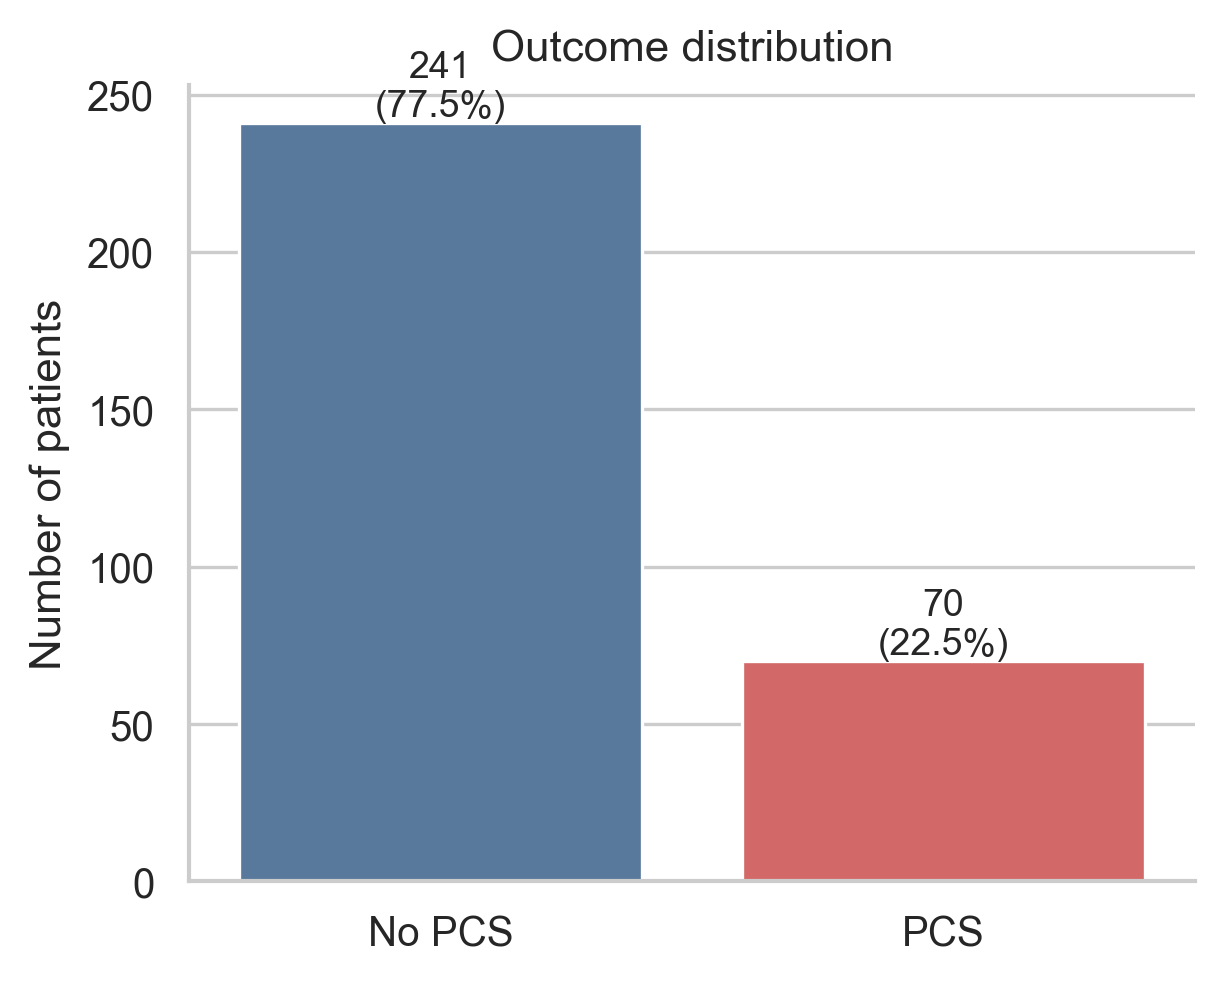
\includegraphics[width=0.48\textwidth]{output/dataset_insights/fig1_outcome_distribution.png}
    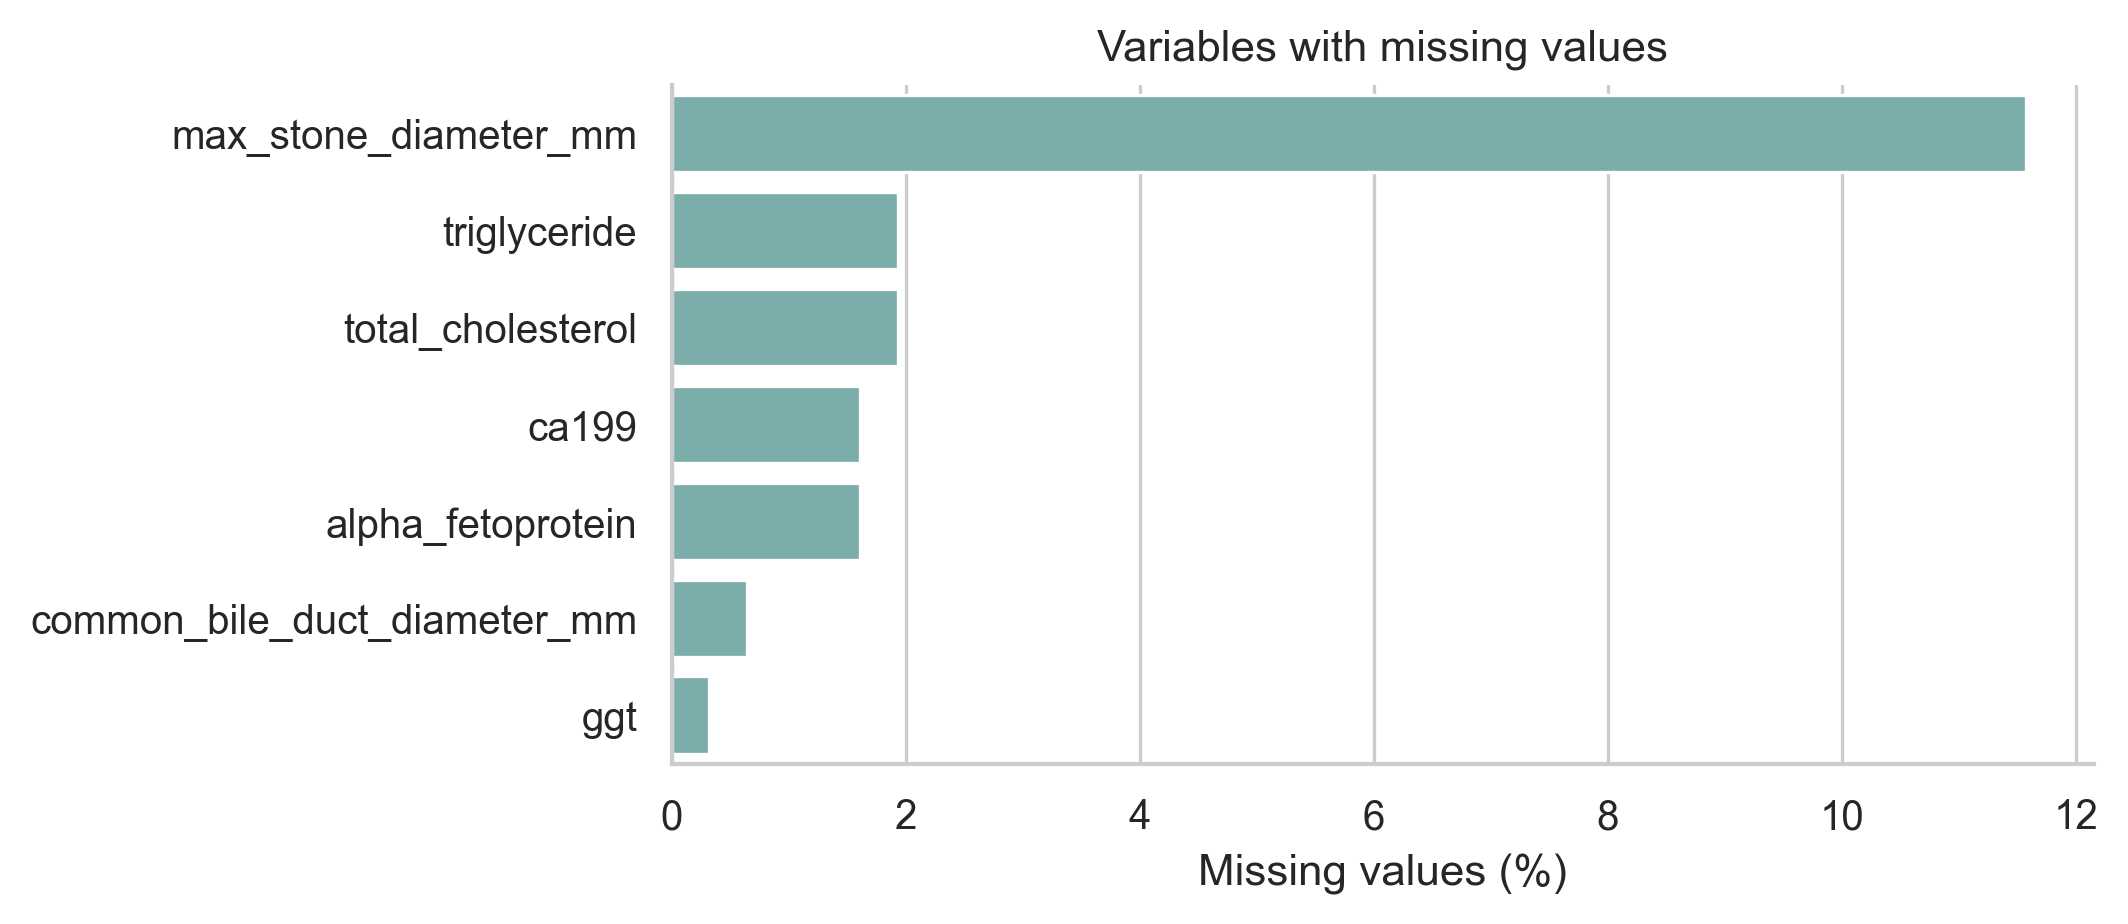
\includegraphics[width=0.48\textwidth]{output/dataset_insights/fig2_missingness_bar.png}
    \caption{Outcome distribution and missingness profile of the de-identified PCS dataset.}
    \label{fig:pcs_dataset_quality}
\end{figure}

\begin{figure}[htbp]
    \centering
    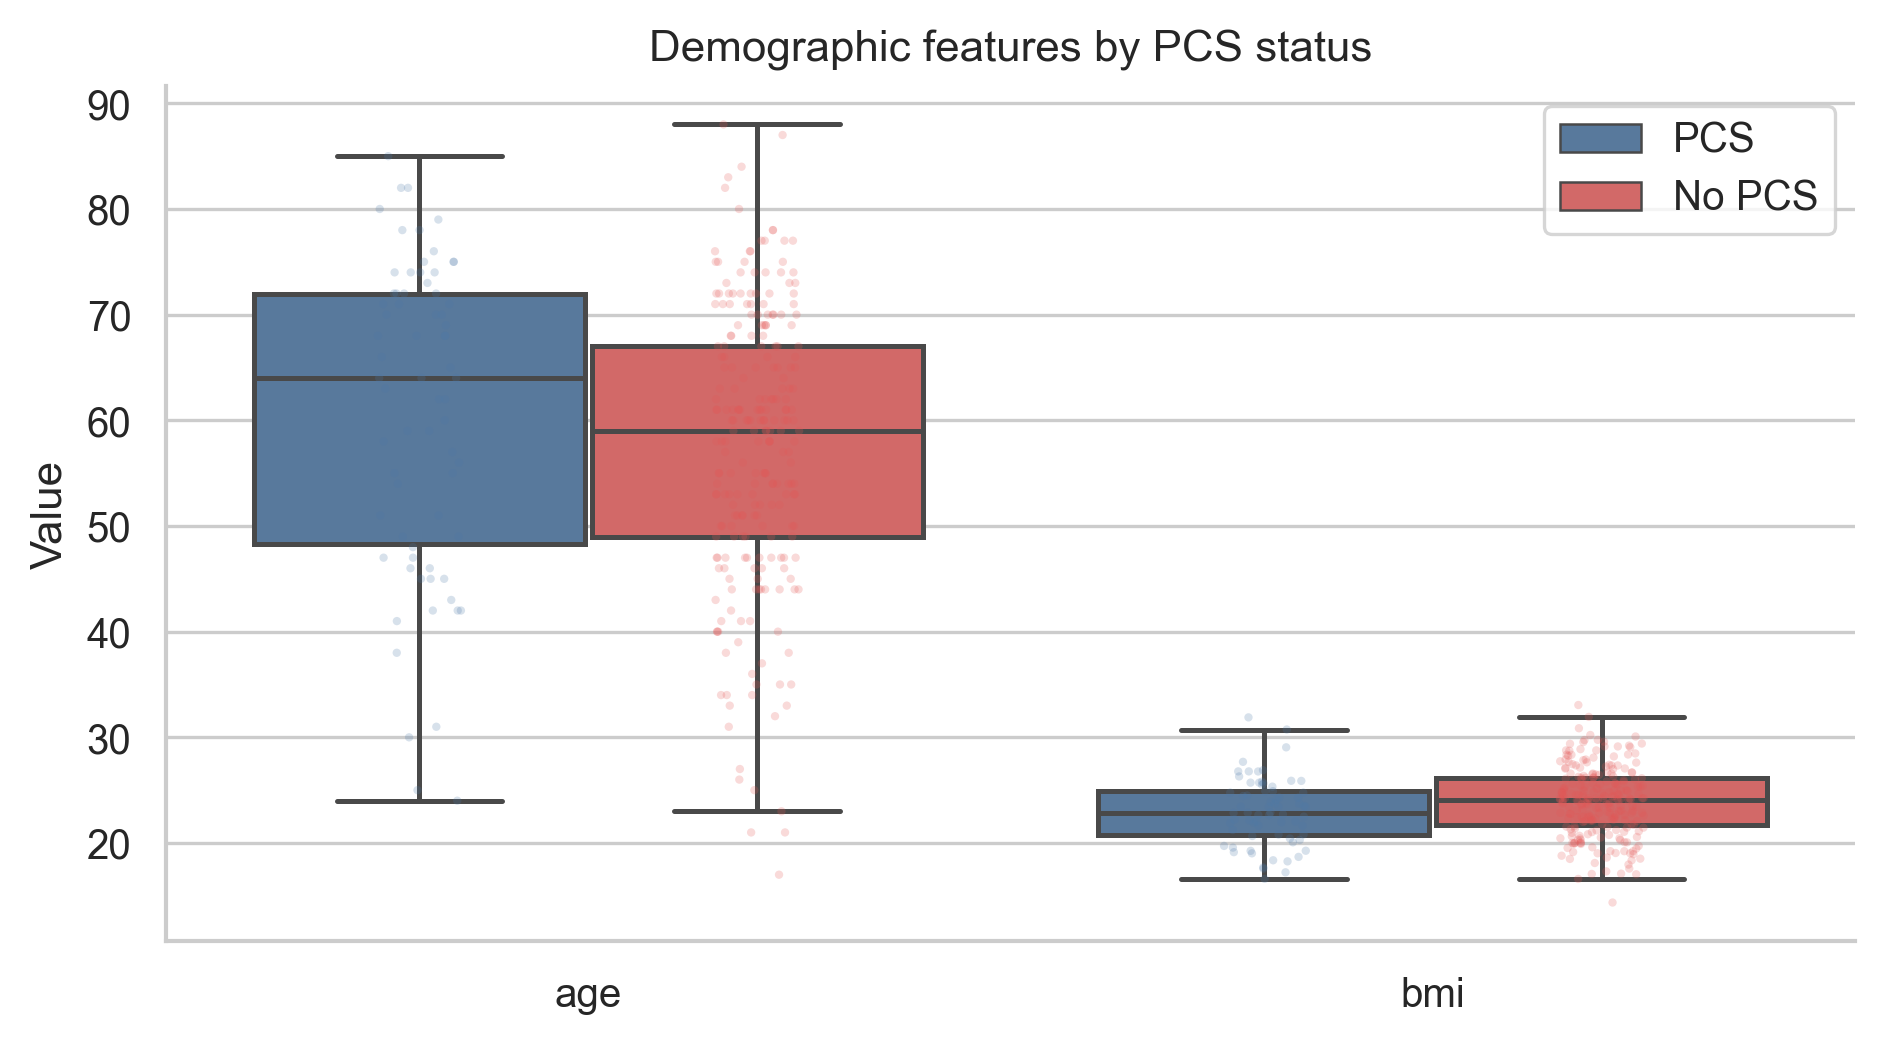
\includegraphics[width=0.48\textwidth]{output/dataset_insights/fig3_demographics_by_pcs.png}
    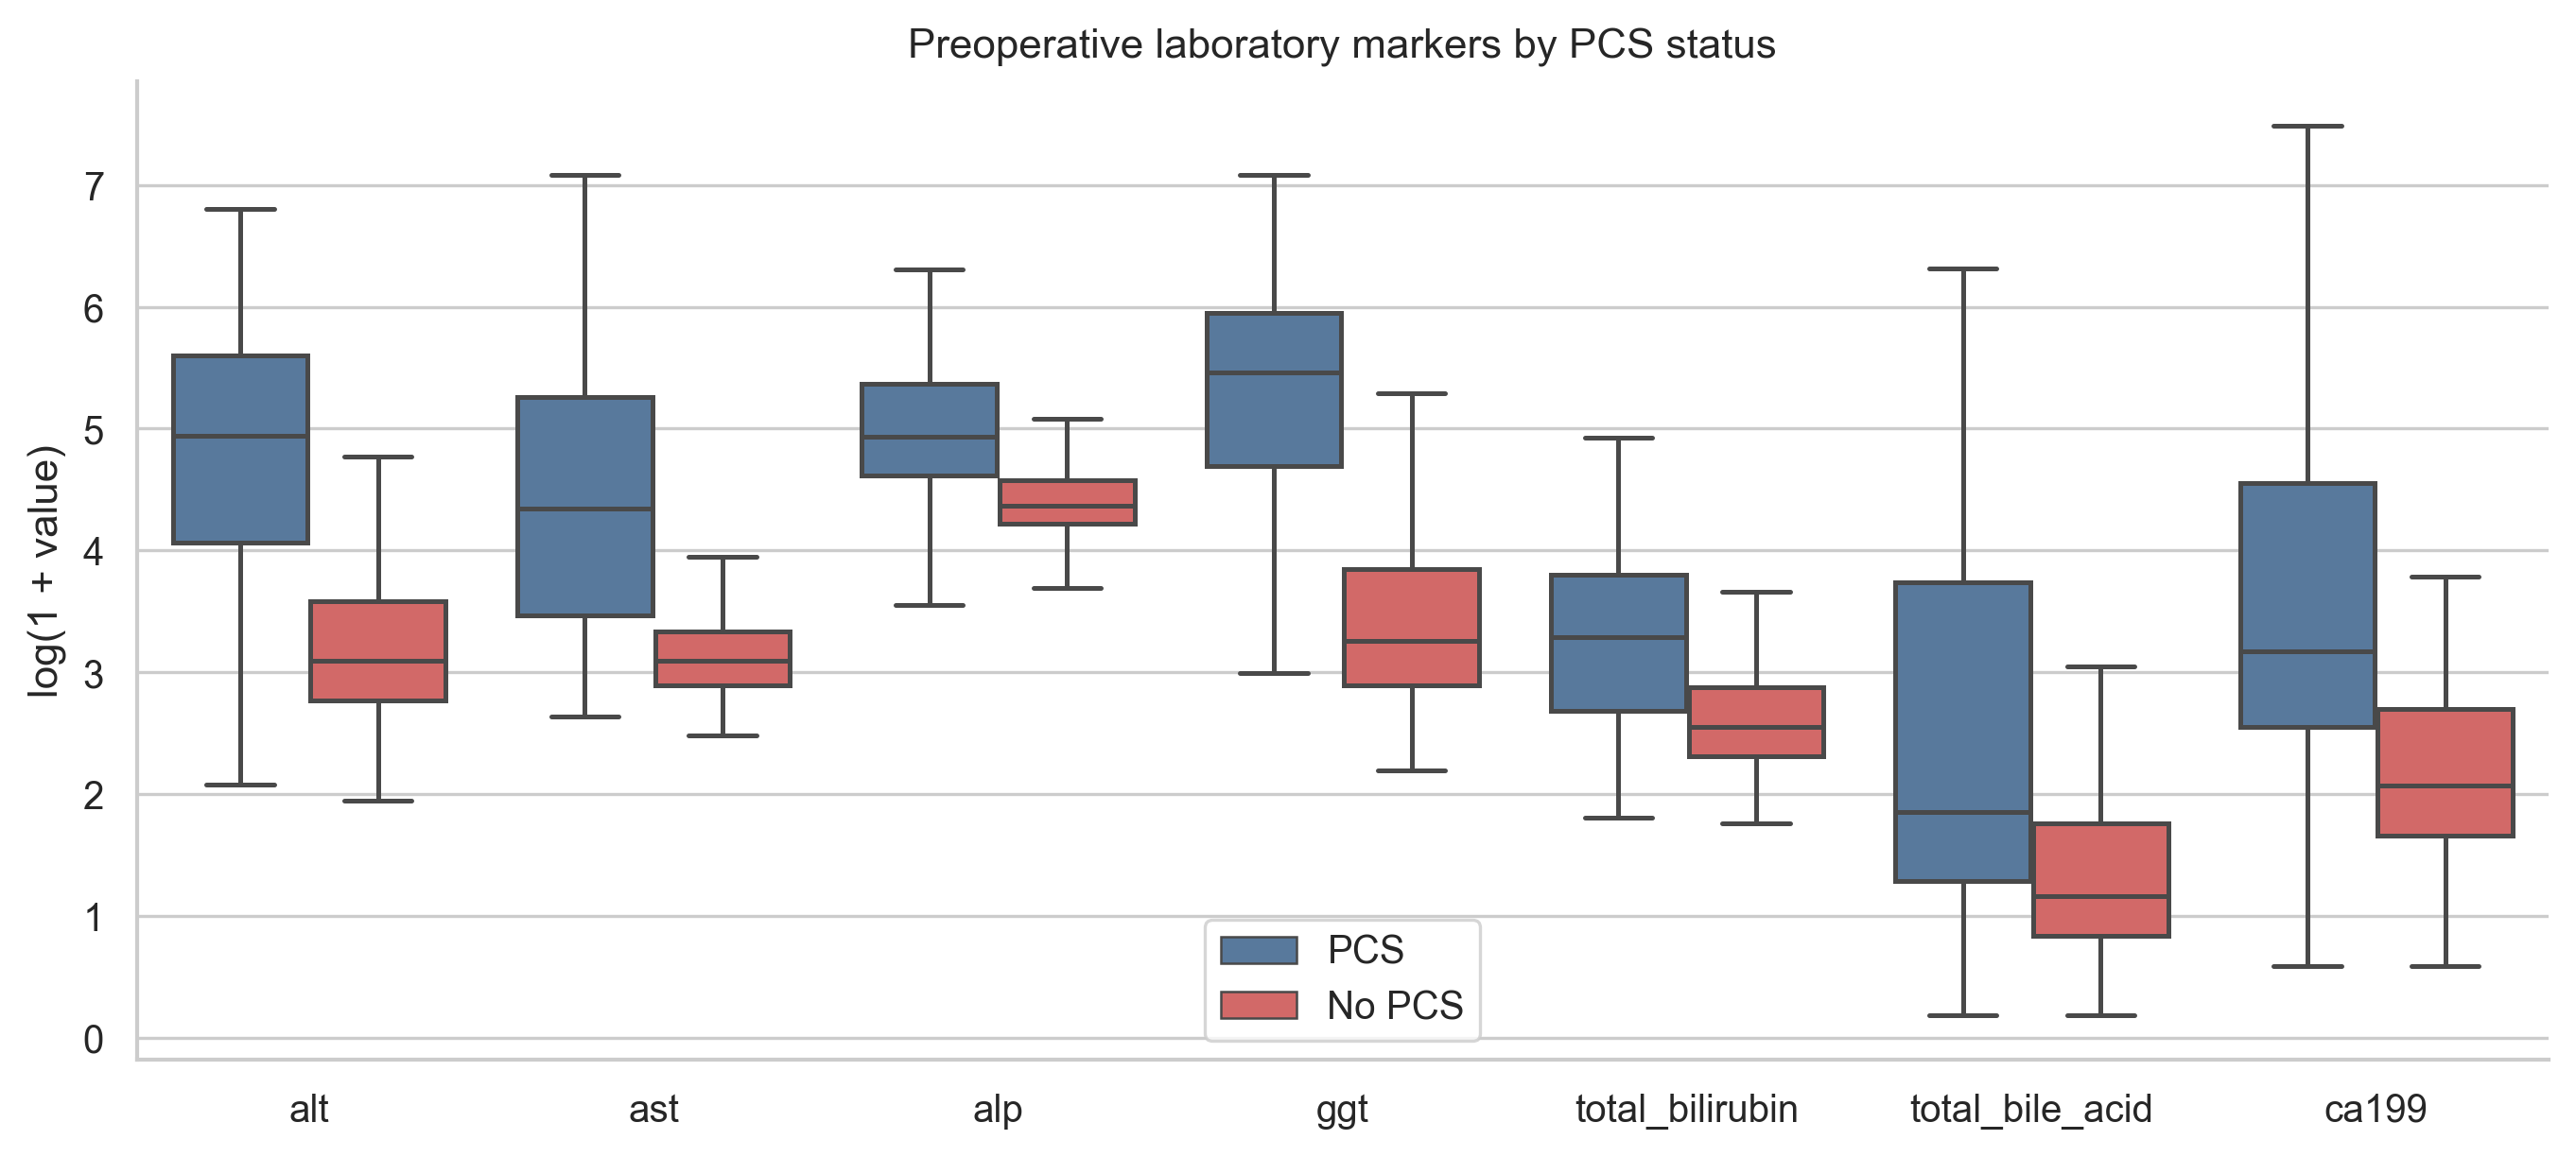
\includegraphics[width=0.48\textwidth]{output/dataset_insights/fig4_lab_markers_by_pcs.png}
    \caption{Distribution of demographic and preoperative laboratory features stratified by PCS status. Laboratory measurements are displayed on a log-transformed scale to reduce the influence of extreme values.}
    \label{fig:pcs_feature_distributions}
\end{figure}

\begin{figure}[htbp]
    \centering
    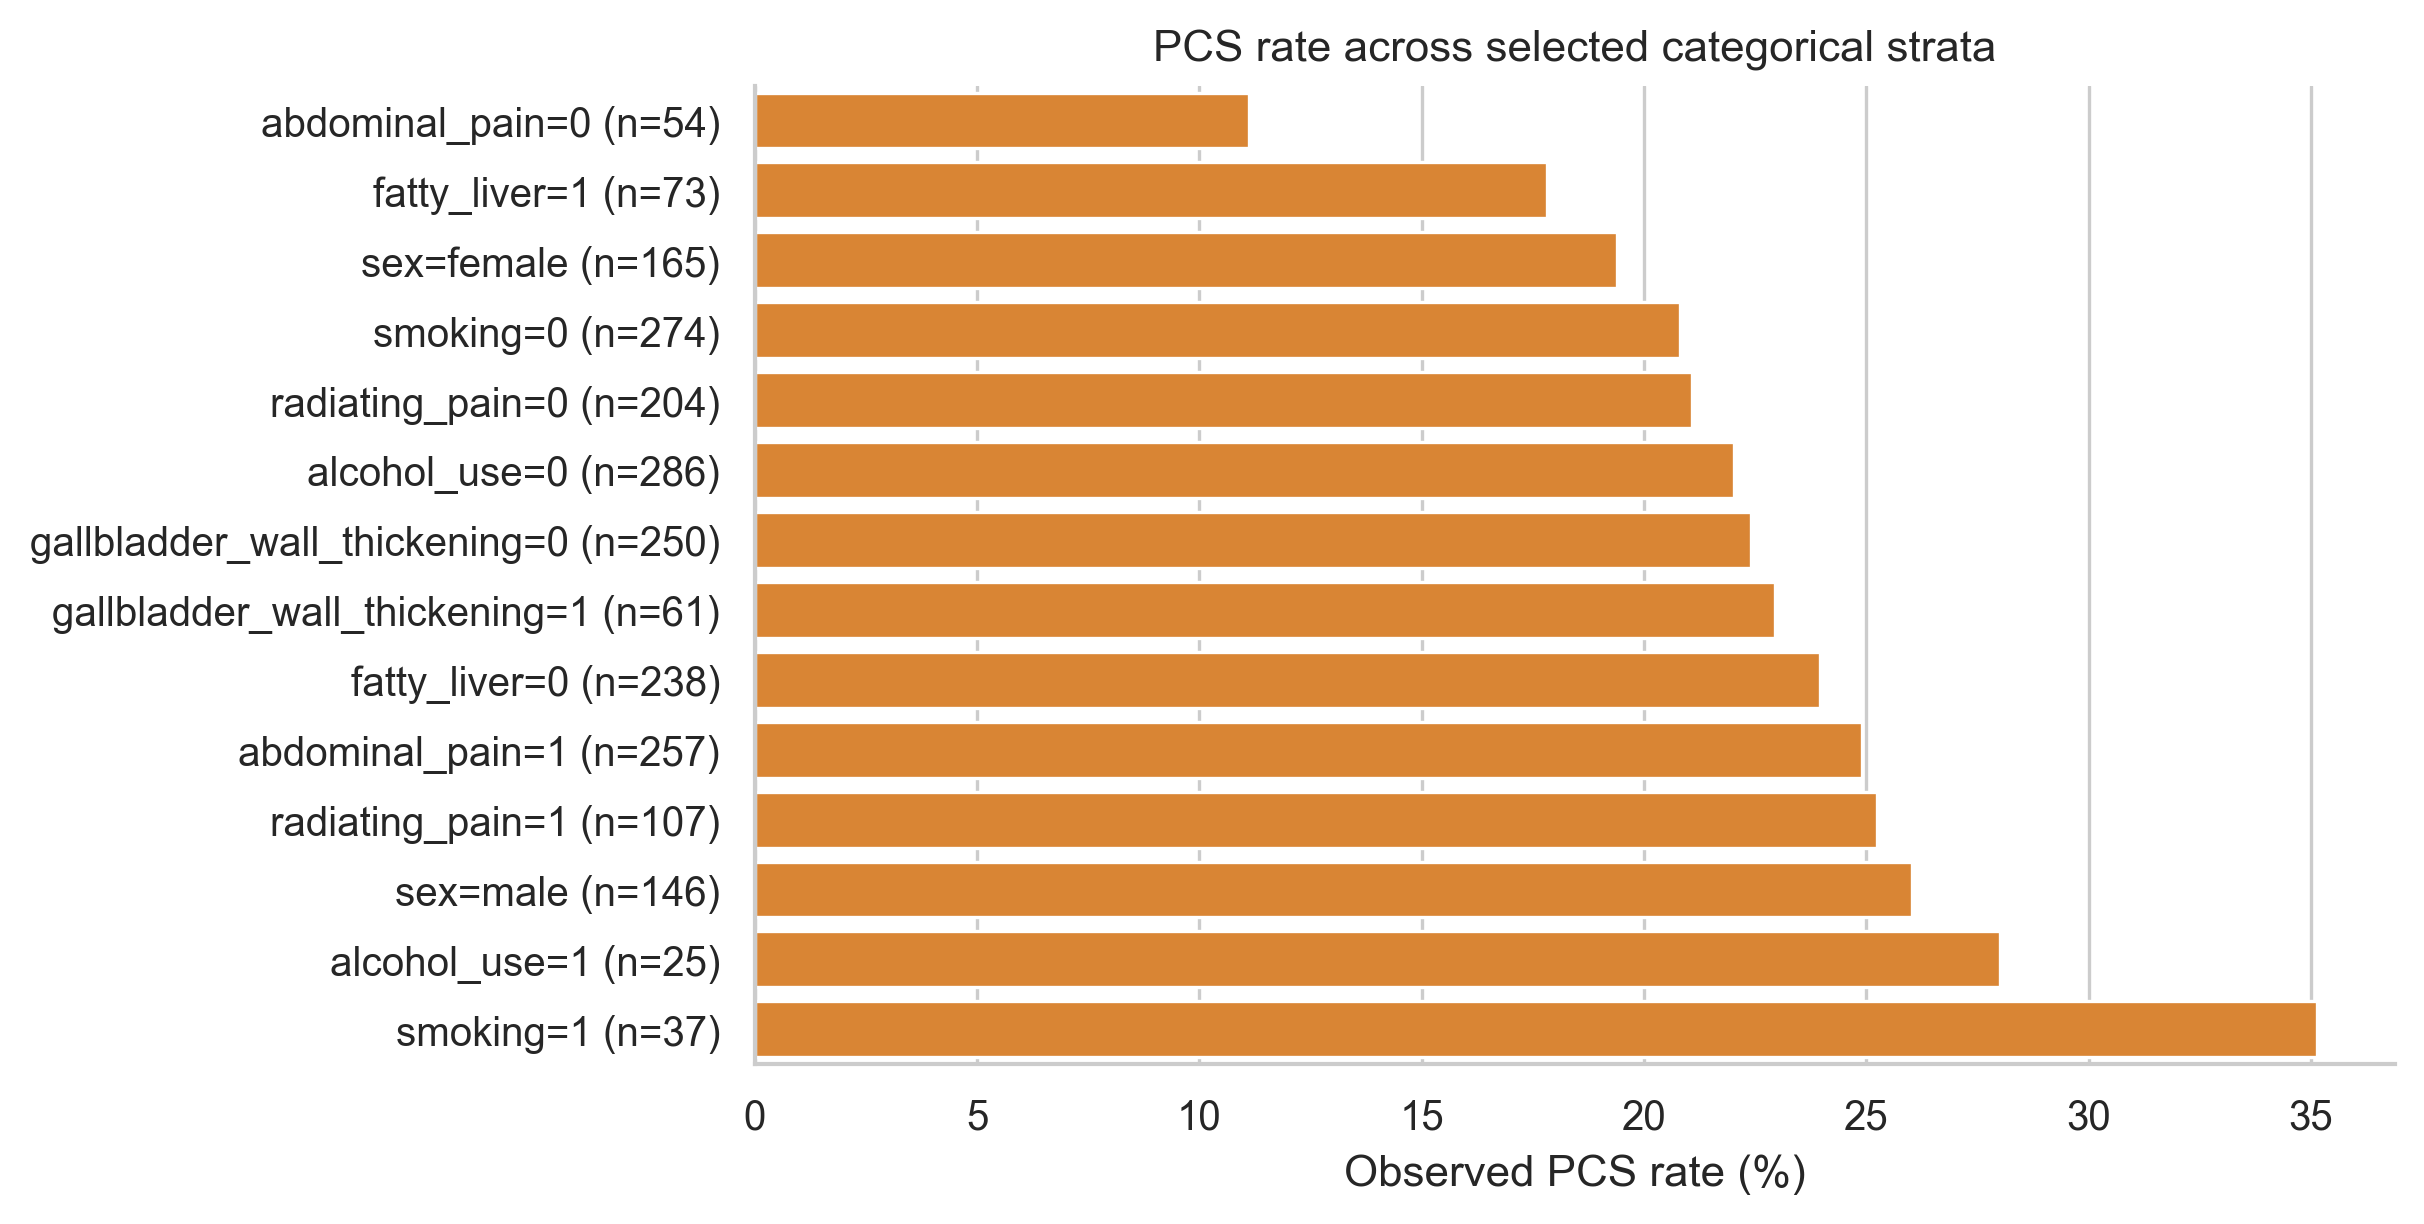
\includegraphics[width=0.48\textwidth]{output/dataset_insights/fig5_categorical_pcs_rates.png}
    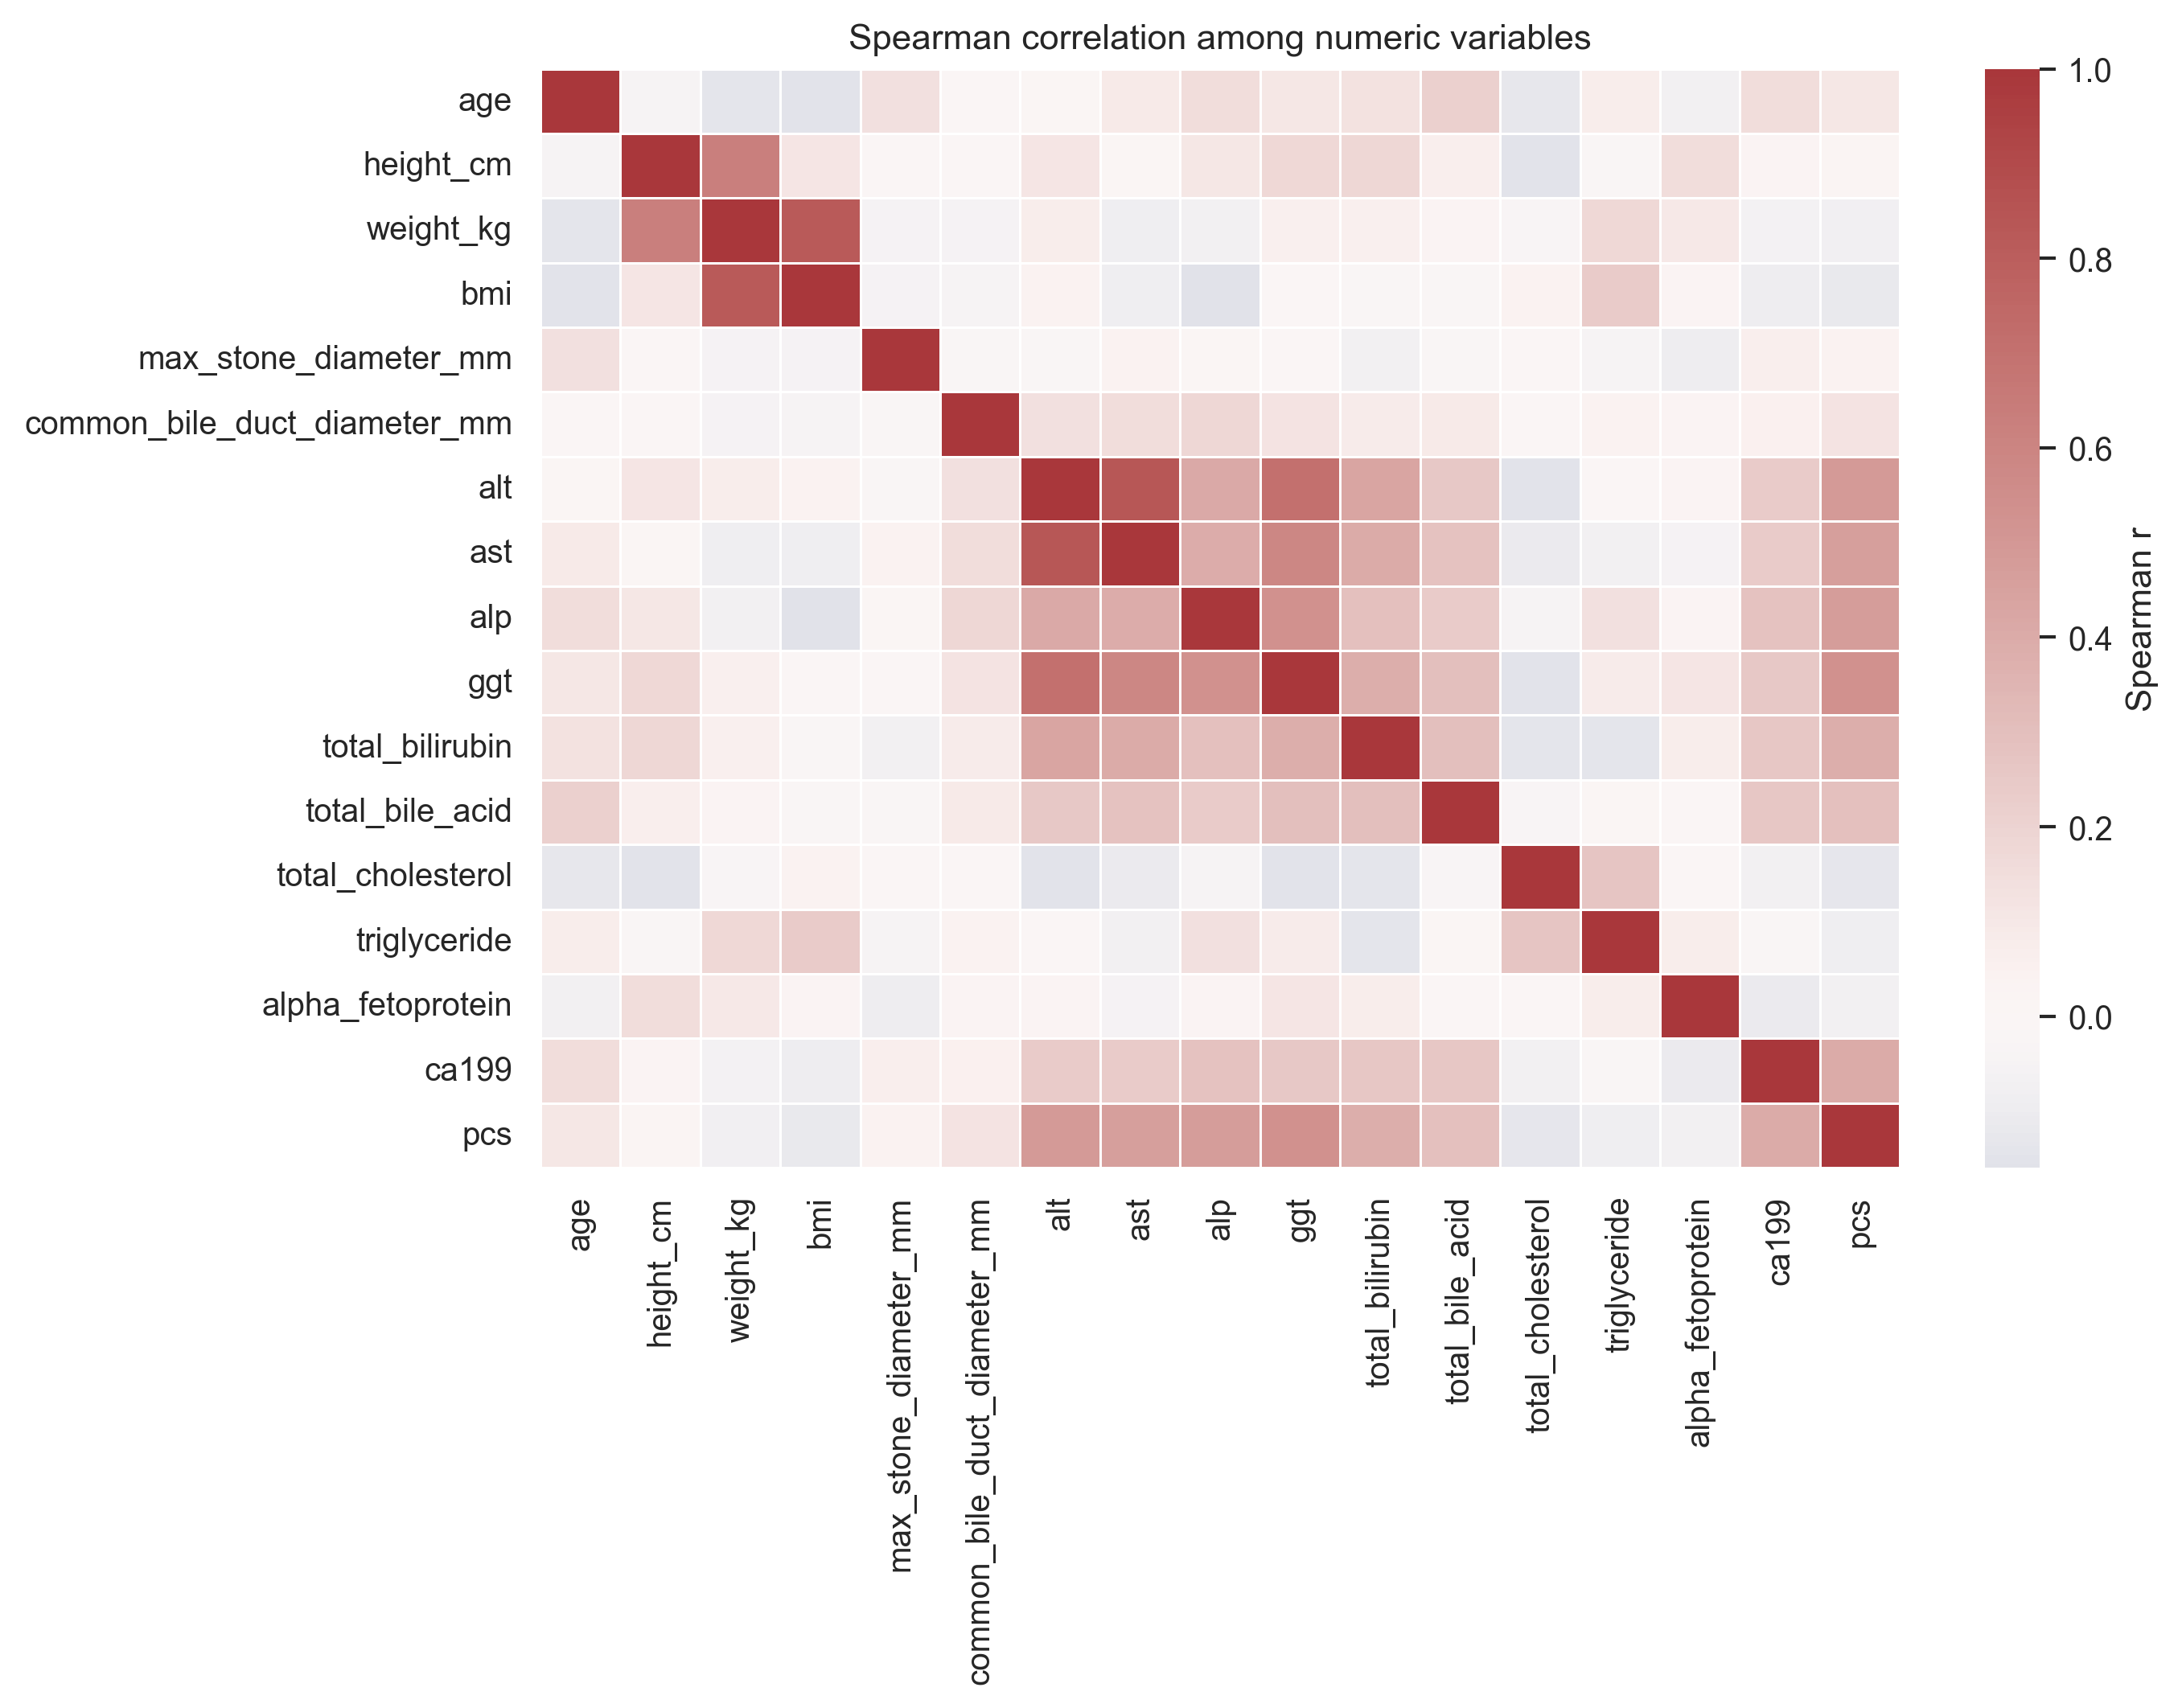
\includegraphics[width=0.48\textwidth]{output/dataset_insights/fig6_numeric_correlation_heatmap.png}
    \caption{Observed PCS rates across selected categorical strata and Spearman correlation structure among continuous variables.}
    \label{fig:pcs_exploratory_analysis}
\end{figure}
